\chapter{Methodik}
\label{chap:Methodik}
% Ziel hier: den Leser in die Lage versetzen, die wesentliche Struktur der Arbeit nachvollziehen zu können (Vorgehen / Geräte / Materialien / Verfahren [also auch Software]  / getroffene Annahmen ... sollten hier erklärt werden)
\section{PCM}\label{sec:pcm}
Die Thermodynamischen Eigenschaften von Eicosane, aufgeführt in Tabelle \ref{tab:eicosane_data}, wurden aus mehreren Quellen entnommen.\\
\begin{table}[H]
  \centering
  \caption{Stoffdaten für Eicosane~\cite{NIST,Nazarychev-2022,Benbrika-2020,Stryker-1990}}\label{tab:eicosane_data}
  \begin{tabular}{|l|l|}
    \hline
    $T_{\text{solidus}}$ & \SI{309}{\kelvin} \\
    \hline
    $T_{\text{liquidus}}$ & \SI{311}{\kelvin} \\
    \hline
    $c_{p,\text{liquid}}$ & \SI{2350.05}{\joule\per\kilogram\per\kelvin} \\
    \hline
    $c_{p,\text{solid}}$ & \SI{2132.4}{\joule\per\kilogram\per\kelvin} \\
    \hline
    $\rho_{\text{solid}}$ & \SI{910}{\kilogram\per\cubic\meter} \\
    \hline
    $\rho_{\text{liquid}}$ & \SI{769}{\kilogram\per\cubic\meter} \\
    \hline
    $\lambda_{\text{liquid}}$ & \SI{0.1505}{\watt\per\meter\per\kelvin} \\
    \hline
    $\lambda_{\text{solid}}$ & \SI{0.4248}{\watt\per\meter\per\kelvin} \\
    \hline
    $\alpha$ & \SI{0.0009}{\per\kelvin} \\
    \hline
    $h_{\text{fus}}$ & \SI{240998.86}{\joule\per\kilogram} \\
    \hline
  \end{tabular}
\end{table}
\begin{figure}[H]
    \centering
    \begin{subfigure}{0.9\textwidth}
        \centering
        \includegraphics[width=\linewidth]{../../Code/pcm_mass.pdf}
        \caption{PCM Masse}\label{fig:pcm_mass}
    \end{subfigure}
    \vspace{1em}  % Optional vertical spacing
    \begin{subfigure}{0.9\textwidth}
        \centering
        \includegraphics[width=\linewidth]{../../Code/pcm_heat_capacity.pdf}
        \caption{PCM Wärmeaufnahme}\label{fig:pcm_heat}
    \end{subfigure}
    \caption{PCM Auslegung}\label{fig:pcm_mass_heat}
\end{figure}
\newpage
\section{Radiator}\label{sec:Radiator}
Hier steht was zu Radiatoren.
\begin{figure}[H]
  \centering
  \includegraphics[width=\linewidth]{../../Code/radiator_leistung.pdf}
  \caption{Radiator Leistung nach Fläche und Temperatur}\label{fig:pcm_heatflux}
\end{figure}
\newpage
\section{PCM-Radiator-Hybrid}\label{sec:pcmRadiatorHybrid}
Eine Hybridlösung wird auch in erwägung gezogen, um die Masse durch Nutzung eines Radiators zu minimieren, wobei wegen aerodynamischer Aufheizung für kurze Zeit ein PCM gebraucht werden könnte.
Um eine umständliche Simulation mittels \ac{cfd} zu vermeiden, wird die Außenkontour der Rakete von Spitze bis Avionik-Sektion, mit Hilfe der Nußelt-Beziehungen, als längsangeströmte ebene Platte angesehen,
wie in Abbildung~\ref{fig:rakete_kontour_zeichnung} dargestellt ist.
Um zu wissen, ob hier die Beziehung für laminare oder turbulente Grenzschichten angewandt werden soll, müssen zunächst die Gültigkeitsbereiche der Reynolds- und Prandtlzahl (\ref{eq:prandtl},~\ref{eq:reynolds}) überprüft werden.
Mittels der Nußelt-Beziehung wird $\alpha$ bestimmt und dann in Gleichung~\ref{eq:qdot} eingesetzt, um auf den spezifischen Wärmestrom zu schließen.
\begin{equation}
  \label{eq:qdot}
  \dot{q} = \alpha \ (T_r - T_w)
\end{equation}
Die Gleichung für laminare Grenzschichten im Gültigkeitsbereich $\text{Re} < \text{Re}_k\\\left(\text{Re}_k \approx 5 \cdot 10^5\right)$ und $0,6 \leq \text{Pr} \leq 2000$ lautet
\begin{equation}
  \label{eq:nusselt_laminar}
  \text{Nu}_x = \frac{\alpha_x x}{\lambda} = 0,332 \ \text{Pr}^{\frac{1}{3}} \ \text{Re}_x^{\frac{1}{2}}
\end{equation}
für turbulente Grenzschichten mit Gültigkeitsbereich: $5 \cdot 10^7 \leq \text{Re}_L \leq 10^7$ und $ 0,6 \leq \text{Pr} \leq 2000$ lautet die Gleichung
\begin{equation}
  \label{eq:nusselt_turbulent}
  \text{Nu}_x = \frac{\alpha_x x}{\lambda} = 0,0296 \ \text{Re}_x^{0,8} \ \text{Pr}^{\frac{1}{3}}
\end{equation}

Für die Reynoldszahl und Prandtlzahl werden die folgenden zwei Gleichungen verwendet
\newline
\noindent\begin{minipage}{.5\linewidth}
\begin{equation}
  \label{eq:reynolds}
  \text{Re}_x = \frac{V \rho x}{\eta}
\end{equation}
\end{minipage}%
\begin{minipage}{.5\linewidth}
\begin{equation}
  \label{eq:prandtl}
  \text{Pr} = \frac{c_p \eta}{\lambda}
\end{equation}
\end{minipage}

Die Dynamische Viskosität wird mittels der Sutherlands-Formel~\ref{eq:dynamische_viskositaet} berechnet, und die Recoverytemperatur mittels der adiabaten Strömungsgleichung.
In diesem Fall wird die Recoverytemperatur statt der Freistromtemperatur benötigt, da die signifikanten Wärmestrome weit über Mach 0.3 stattfinden.
\begin{equation}
  \label{eq:dynamische_viskositaet}
  \eta = \eta_0 \frac{T_0 + C}{T_{\infty} + C} {\left( \frac{T_{\infty}}{T_0} \right)}^{\frac{2}{3}}
\end{equation}
\begin{equation}
  \label{eq:recovery_temperatur}
  T_r = T_{\infty} \left( 1 + r \frac{\kappa + 1}{2} \text{Ma}^2 \right)
\end{equation}
Der Recovery-Faktor kann mittels der folgenden Gleichung approximiert werden
\begin{equation}
  \label{eq:recovery_faktor}
  r = \frac{2}{\left(\kappa - 1\right) \text{Ma}_e^2} \left(\frac{T_{a_{w}}}{T_e} - 1\right) \approx
  \begin{cases}
    \sqrt[3]{\text{Pr}} & \text{für turbulente Grenzschicht}\\
    \sqrt{\text{Pr}} & \text{für laminare Grenzschicht}
  \end{cases}
\end{equation}
\newpage
% Hybrid PCM ohne aufheizung
\begin{figure}
  \centering
  \begin{tikzpicture}[rotate border/.style={shape border uses incircle, shape border rotate=#1}, scale=0.8]
    \draw[thick] (3,3) -- (3,-1) -- (9,-1) -- (9,3);
    \draw[thick] (3,3) -- node [midway, above] {Avionik Sektion}  (9,3);
    \draw[thick] (4,3) -- (4,-1); % PCM Lamellen
    \draw[thick] (3,-0.5) -- (4,-0.5);
    \draw[thick] (3,0) -- (4,0);
    \draw[thick] (3,0.5) -- (4,0.5);
    \draw[thick] (3,1) -- (4,1);
    \draw[thick] (3,1.5) -- (4,1.5);
    \draw[thick] (3,2) -- (4,2);
    \draw[thick] (3,2.5) -- (4,2.5);
    \node at (-0.5,2) [style={single arrow, draw}, minimum height=3cm, minimum width=0.5cm, thick]{$\dot{Q}_{\mathrm{Umwelt}}$}; % Wärmestrom pfeil
    \node at (-0.5,0) [style={single arrow, draw}, minimum height=4.5cm, minimum width=1.5cm, shape border rotate=180, thick]{$\dot{Q}_{\mathrm{Radiator}}$}; % Wärmestrom pfeil
    \node at (6.5,1)[style={single arrow, draw}, minimum height=3cm, minimum width=0.5cm, shape border rotate=180, thick]{$\dot{Q}_{\mathrm{Avionik}}$}; % Wärmestrom pfeil
    \draw[->, thick, -{Stealth[length=0.25cm]}] (1,3.75) node [above=1pt] {PCM mit Lamellen} -- (3.5,2.6);
  \end{tikzpicture}
  \caption{PCM Wärmestrom ohne aerodynamische Aufheizung}\label{fig:pcm_waermestrom_diagramm}
\end{figure}
$\dot{Q}_{\mathrm{Radiator}} = \dot{Q}_{\mathrm{Umwelt}} + \dot{Q}_{\mathrm{Avionik}}$ In diesem Fall reicht die Leistung des Radiators, um die Avionik auf Betriebstemperatur zu halten.
% Hybrid PCM Wärmestrom bei aufheizung
\begin{figure}[H]
  \centering
  \begin{tikzpicture}[rotate border/.style={shape border uses incircle, shape border rotate=#1}, scale=0.8]
    \draw[thick] (3,3) -- (3,-1) -- (9,-1) -- (9,3);
    \draw[thick] (3,3) -- node [midway, above] {Avionik Sektion}  (9,3);
    \draw[thick] (4,3) -- (4,-1); % PCM lamellen
    \draw[thick] (3,-0.5) -- (4,-0.5);
    \draw[thick] (3,0) -- (4,0);
    \draw[thick] (3,0.5) -- (4,0.5);
    \draw[thick] (3,1) -- (4,1);
    \draw[thick] (3,1.5) -- (4,1.5);
    \draw[thick] (3,2) -- (4,2);
    \draw[thick] (3,2.5) -- (4,2.5);
    \node at (-0.5,2) [style={single arrow, draw}, minimum height=4.5cm, minimum width=1.5cm, thick]{$\dot{Q}_{\mathrm{Umgebung}}$}; % Wärmestrom pfeil
    \node at (-0.5,0) [style={single arrow, draw}, minimum height=4.5cm, minimum width=1.5cm, shape border rotate=180, thick]{$\dot{Q}_{\mathrm{Radiator}}$}; % Wärmestrom pfeil
    \node at (6.5,1)[style={single arrow, draw}, minimum height=3cm, minimum width=0.5cm, shape border rotate=180, thick]{$\dot{Q}_{\mathrm{Avionik}}$}; % Wärmestrom pfeil
  \end{tikzpicture}
  \caption{PCM Wärmestrom bei aerodynamischer Aufheizung}\label{fig:pcm_waermestrom_aufheizung_diagramm}
\end{figure}
Hier reicht die Leistung des Radiators nicht mehr aus und das \ac{pcm} fängt an zu schmilzen. Zu beachten ist,
dass die Leistung des Radiators durch die Temperaturerhöhung steigen würde, wegen des \ac{pcm} jedoch sehen wir das System als isotherm an.
% Raketenkontour im Luftstrom für ebene Platte Annahme
\begin{figure}[H]
  \centering
  \begin{tikzpicture}
    \draw[thick] (0,0) arc [start angle=90, end angle=270, x radius=5cm, y radius= 1.5cm]; %nosecone
    \draw[thick] (0,0) -- (3,0); % hülle
    \draw[thick] (0,-3) -- (3,-3); % hülle
    \draw[thick] (-5.75,-1.5) -- (-5.25,-1.5); % maß links
    \draw[thick] (1,0.25) -- (1,0.75); % maß rechts
    \draw[thick] (0,0.5) arc [start angle=90, end angle=180, x radius=5.5cm, y radius= 2cm]; % maß bogen
    \draw[thick] (0,0.5) -- node [near start, above] {Länge} (1,0.5); % maß grade sektion
    \draw[->, thick, -{Stealth[length=0.25cm]}] (-10,0.5) -- node [midway, above] {Luftstrom} (-7,0.5); % free stream pfeile
    \draw[->, thick, -{Stealth[length=0.25cm]}] (-10,-0.5) -- (-7,-0.5); % Strompfeile
    \draw[->, thick, -{Stealth[length=0.25cm]}] (-10,-1.5) -- (-7,-1.5);
    \draw[->, thick, -{Stealth[length=0.25cm]}] (-10,-2.5) -- (-7,-2.5);
    \draw[->, thick, -{Stealth[length=0.25cm]}] (-10,-3.5) -- (-7,-3.5);
    \draw[thick] (0,0) -- (0,-2.5); % casing wall
    \draw[thick] (2,0) -- (2,-2.5); % casing wall
    \draw[thick] (0,-2.5) -- (2,-2.5); % casing bottom
    \node at (1,-1.5) [style={single arrow, draw}, minimum height=0.5cm, minimum width=1.5cm, rotate=90, thick]{$\dot{Q}_{\mathrm{Avionik}}$}; % Wärmestrom pfeil
  \end{tikzpicture}
  \caption{Kontourlänge vom Staupunkt der Rakete bis zum Mittelpunkt des Radiators}\label{fig:rakete_kontour_zeichnung}
\end{figure}
In Abbildung~\ref{fig:dimensionierung_ablauf} sieht man wie die Dimensionierung in den Programmen abläuft. Die Programme erzeugen alle Graphen und rechnen simultan für gegebenen Avionik Wärmestrom alle Werte aus.
\begin{figure}[H]
  \centering
  \begin{tikzpicture}[
    sibling distance=10em,
    every node/.style = {
      shape=rectangle,
      rounded corners,
      draw,
      align=center,
      minimum width=3cm
    },
    edge from parent/.style = {
      draw,
      ->,
      -{Stealth[length=0.25cm]},
      thick
    },
    arrow/.style = {
      ->,
      -{Stealth[length=0.25cm]},
      thick
    }
  ]

    % Top nodes
    \node (avionik) at (-2.1, 4) {Avionik Wärmestrom};
    \node (sonne)   at ( 2.1, 4) {Sonne Wärmestrom};

    % Radiator Fläche centered below
    \node (radiator) at (0, 2) {Radiator Fläche};

    % Children of Radiator
    \node (breite) at (-2.1, 0) {PCM Breite};
    \node (aerothermal) at (2.1, 0) {Aerothermal Wärmestrom};

    % PCM Kapazität as a separate node (not a child directly)
    \node (kapazitaet) at (2.1, -2) {PCM Kapazität};

    % PCM Höhe node below the center of breite and kapazitaet
    \node (hoehe) at (0, -4) {PCM Höhe};
    \node (gewicht) at (0, -6) {PCM Gewicht};

    % Arrows
    \draw[arrow] (avionik) -- (radiator);
    \draw[arrow] (sonne) -- (radiator);
    \draw[arrow] (radiator) -- (breite);
    \draw[arrow] (radiator) -- (aerothermal);
    \draw[arrow] (aerothermal) -- (kapazitaet);
    \draw[arrow] (breite) -- (hoehe);
    \draw[arrow] (kapazitaet) -- (hoehe);
    \draw[arrow] (hoehe) -- (gewicht);

  \end{tikzpicture}
  \caption{Dimensionierungs-Ablauf in der Vorauslegung}\label{fig:dimensionierung_ablauf}
\end{figure}
\newpage
\section{Thermales Interface}\label{thermalesInterface}
Hier gehts jetzt um wie die wärme verteilt und abtransportiert wird. Laut~\cite{Xingcun-2011} seite 35 geht die meiste Wärme in die PCB.
\newpage
\subsection{Thermal Straps}\label{thermalstraps}
Um das \ac{pcb} mit der Heatpipe zu verbinden werden Thermal Straps aus verschiedenen Materialien analysiert.
Thermal Straps sind flexible Verbindungsteile die Wärmebrücken zwischen mehreren Bauteilen gewehrleisten.
Wegen der hohe Wärmeleitzahl von \ac{pgs} und bedonders für Thermal Straps wichtigen Flexibilität, sind diese eine interessante Option.
Ein Nachteil von \ac{pgs} ist die geringe Dicke und der daraus resultierende geringe Querschnitt, welcher trotz hoher Wärmeleitzahl zu hoher Wärmestromdichte und stärkerer Temperaturerhöhung führen kann.
Im Vergleich mit herkömmlichen Materialien wie Aluminium und Kupfer soll ein Vergleich gezogen werden.
\begin{figure}[H]
  \centering
  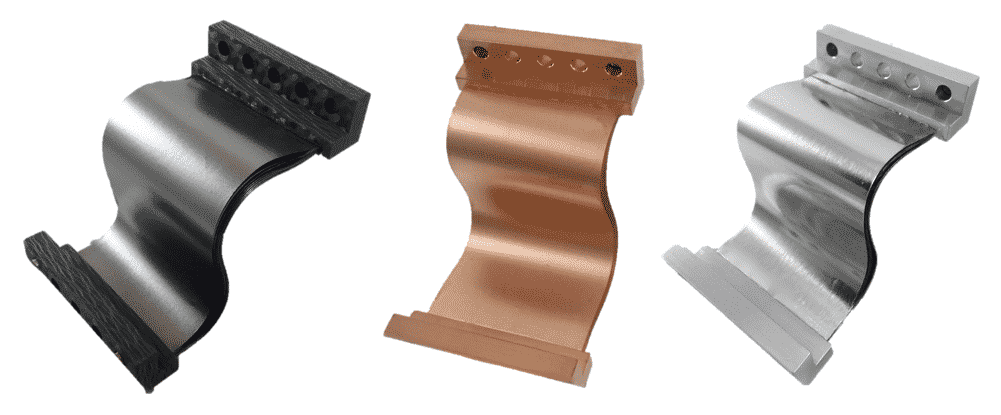
\includegraphics[width=\textwidth]{thermal_straps_commercial.png}
  \caption{Kommerzeill erhältliche Thermal Straps aus Graphen, Kupfer und Aluminium der Firma Thermal Space and Thermal Straps}\label{fig:thermalstraps_commercial}
\end{figure}
\newpage
\section{CFD}\label{cfd}
\begin{figure}[H]
  \centering
  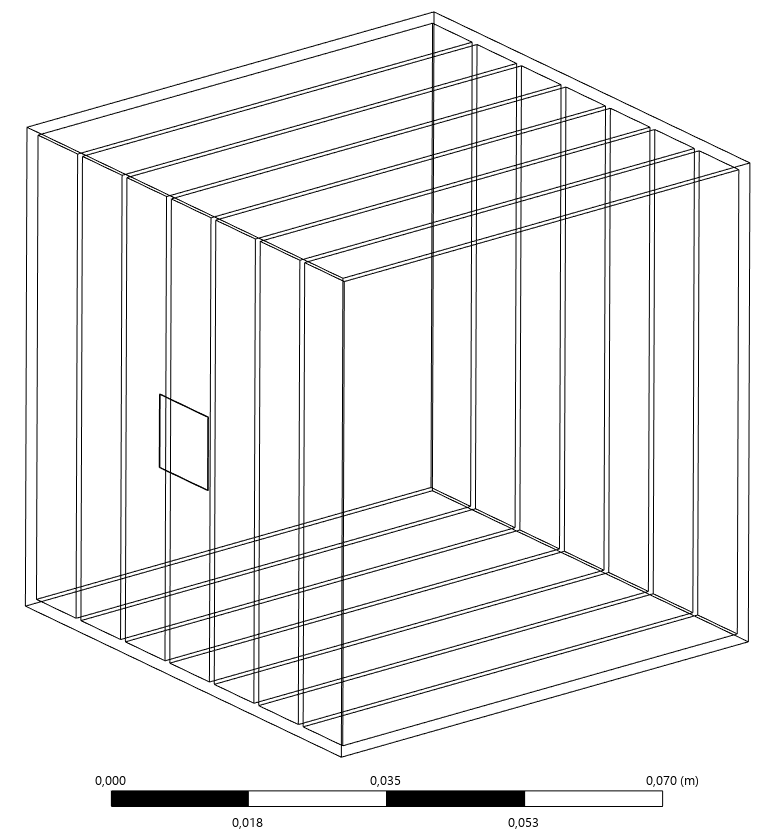
\includegraphics[width=\textwidth]{40WPCM_struktur.png}
  \caption{\ac{pcm} Struktur}\label{pcmstruktur}
\end{figure}
\begin{figure}
  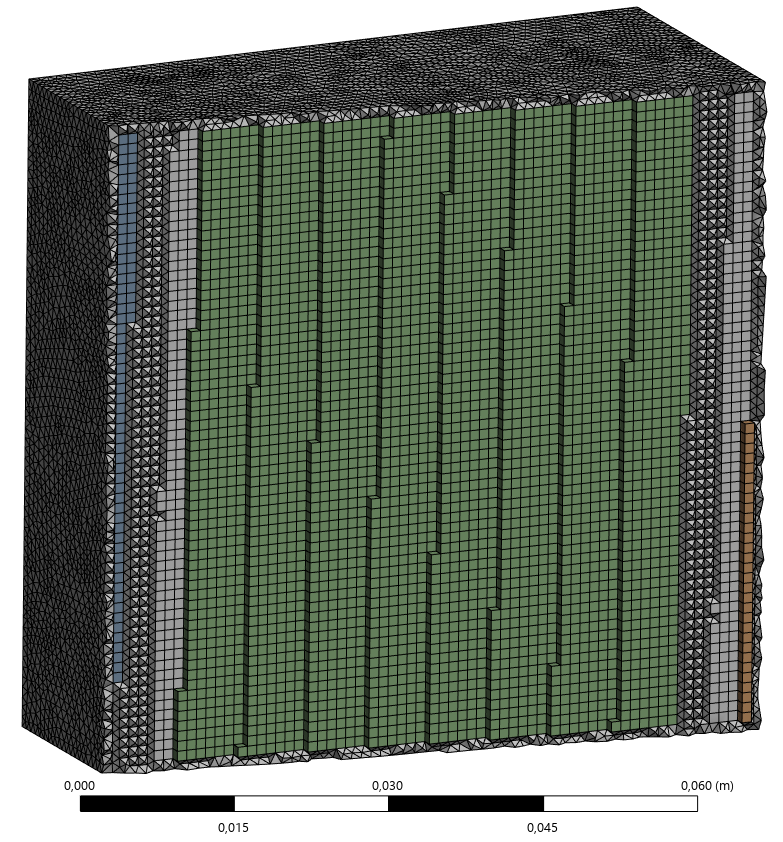
\includegraphics[width=\textwidth]{40WPCM_mesh1.png}
  \caption{\ac{pcm} Mesh}\label{pcmmesh}
\end{figure}
%recoverytemperatur wahrscheinlich richtig noch recherchieren